\chapter{La scheda Nexys4 DDR}

\begin{figure}[h!]
	\centering
	\def\svgwidth{\columnwidth}
	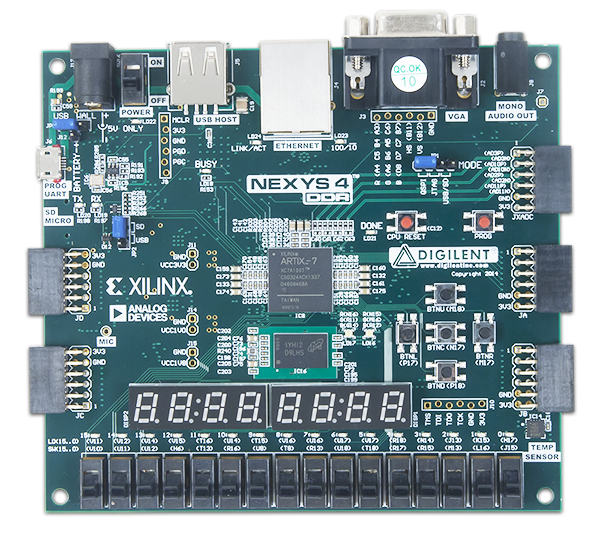
\includegraphics[width=0.6\columnwidth]{TeX_files/nexys4_ddr.png}
    \caption{Scheda Digilent Nexys4 DDR.}
\end{figure}

L'hardware utilizzato per il progetto consiste in una scheda Nexys4 DDR.
Il nucleo della scheda è costituito da un FPGA Xilinx Artix 7 XC7A100T.
Attorno ad esso sono collegati vari connettori, sensori e pulsanti\cite{nexys4referencemanual}.

Per la realizzazione del sintetizzatore si farà uso dei seguenti componenti:
\begin{itemize}
    \item \textbf{Bridge USB-UART} Il bridge USB<->UART permette la lettura
          dei messaggi MIDI, inviati dal computer attraverso la porta seriale
    \item \textbf{Mono Audio Output} Un connettore audio monofonico di tipo minijack 
          viene usato per emettere il suono.
    \item \textbf{Clock Crystal} Il cristallo che fornisce un clock di \SI{100}{\mega\hertz}
          alla FPGA e alla scheda.
\end{itemize}

L'output fornito dal jack audio viene generato attraverso un convertitore analogico/digitale,
costituito da un filtro passa-basso a cui viene fornito in ingresso il segnale
da generare in codifica PWM.

Il filtro passabasso è un filtro di Butterworth del quarto ordine, la cui risposta
in frequenza è rappresentata nella \cref{fig:freq_resp}
\begin{figure}[h!]
	\centering
	\def\svgwidth{\columnwidth}
	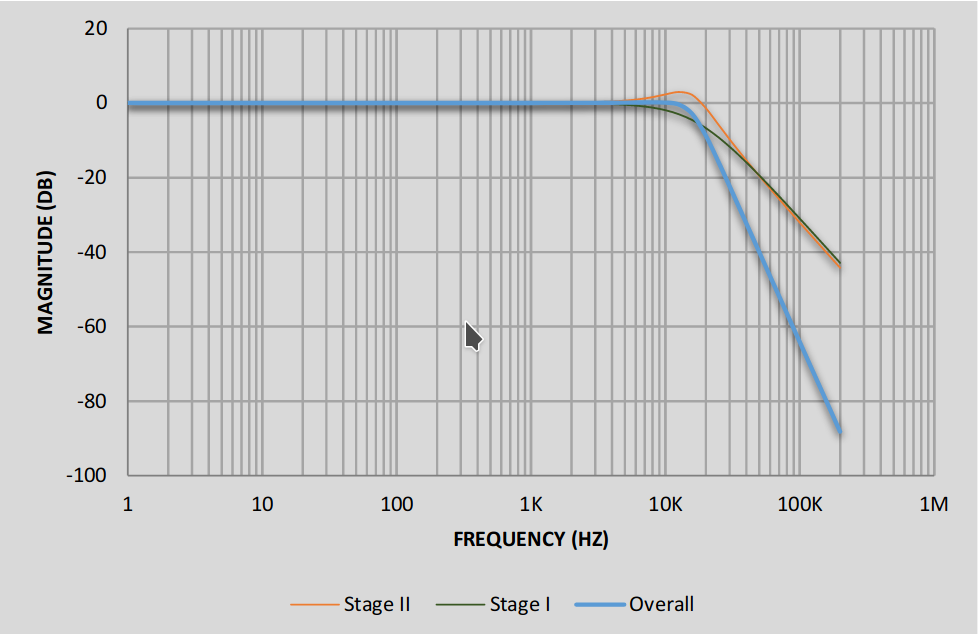
\includegraphics[width=0.6\columnwidth]{TeX_files/freq_response.png}
    \caption{Risposta in frequenza del filtro passa-basso prima dell'uscita audio}
    \label{fig:freq_resp}
\end{figure}

\section{FPGA}
Una Field-programmable Gate Array (FPGA) è un circuito digitale integrato
capace di implementare le più svariate funzioni in modo programmatico:
può essere utilizzato per la fase di prototipazione di Application-specific
Integrated Circuits (ASIC), oppure per sostituirli nel caso in cui i costi
di integrazione di una FPGA nel progetto siano minori dei costi di sviluppo
e realizzazione dell'ASIC (che di solito sono più vantaggiosi per volumi
di produzione molto grandi).
Un FPGA, data la sua natura generale, offre performance inferiori sia
in consumi che in prestazioni rispetto ad un ASIC, ma ha come vantaggio
la riprogrammabilità (anche una volta integrato nel progetto), che
è invece impossibile con un circuito integrato specifico. 
Un altro uso che si va affermando negli ultimi anni è l'utilizzo dei
FPGA come acceleratori software, ad esempio per applicazioni di 
trading finanziaro e intelligenza artificiale.

\subsection{Struttura di un FPGA}
Una FPGA ha una struttura regolare e contiene:
\begin{itemize}
    \item \textbf{configurable logic blocks}: in breve \textbf{CLB}, blocchi
            logici configurabili che permettono di realizzare funzioni
            logiche arbitrarie
    \item \textbf{configurable routing}: i blocchi logici sono collegati
          attraverso delle connessioni a loro volta configurabili,
          rendendo possibile creare funzioni logiche a un maggior numero
          di ingressi e più complesse
\end{itemize}

Oltre a queste due componenti fondamentali, una FPGA contiente altri
componenti necessari al suo funzionamento e interfacciamento con
circuiti esterni.
L'FPGA utilizzato dalla scheda Nexys 4 DDR è uno Xilinx Artix 7 XC7A100T
e contiene svariati blocchi\cite{artix7overview}, tra cui:

\begin{itemize}
    \item \textbf{I/O blocks}: blocchi di input e output,
           permettono alla FPGA di interfacciarsi con l'esterno
    \item \textbf{DSP blocks}: blocchi che rendono più efficiente in termini
           di risorse l'implementazione di sommatori e moltiplicatori
    \item \textbf{Memory blocks}: è possibile trovare anche blocchi di
           memoria all'interno di una FPGA
    \item \textbf{Clock Management Tiles}: oltre a contenere la circuiteria
            necessaria per la gestione e propagazione del segnale di clock,
            permettono operazioni avanzate sul segnale di clock come la
            generazione di clock a frequenze diverse o di clock sfasati
    \item \textbf{Dedicated blocks}: Blocchi contenenti funzionalità avanzate,
            come ad esempio l'interfaccia PCI Express e blocchi di I/O ad alta
            velocità
\end{itemize}

Esso contiene 101440 logic elements (i blocchi elementari di un CLB), e sei
clock management tiles (CMT) con phase-locked loop.
Di importanza per il progetto trattato sono i 240 DSP slices, 
data la presenza di molti sommatori all'interno del design,
 e i 4860 Kbits di Block Ram (BRAM) che vengono impiegati in fase di 
sintesi per memorizzare sia la forma d'onda campionata che
le frequency tuning words impiegate nella digital direct synthesis.

\begin{figure}[H]
	\centering
	\def\svgwidth{\columnwidth}
	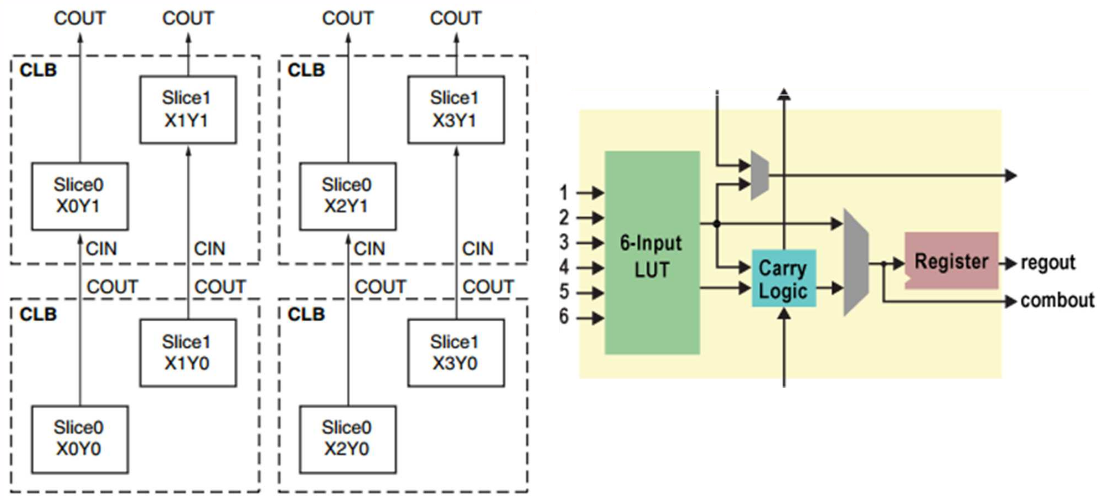
\includegraphics[width=0.8\columnwidth]{TeX_files/CLB.png}
    \caption{Struttura gerarchica di una FPGA: a sinistra l'insieme di più CLB,
    a destra la struttura di un singolo logic element}
\end{figure}
\subsection{Struttura di un CLB}
Il CLB è la macrostruttura fondamentale di una FPGA.
I circuiti elementari all'interno di un CLB sono i logic elements, che implementano
con una look-up table (LUT) una funzione logica a 5 o 6 ingressi.
Alcune LUT sono utilizzabili anche come elementi di sola memorizzazione.
Ogni logic element contiene anche un elemento di memoria in cui poter memorizzare il risultato
dell'operazione, configurabile sia come flip-flop che come latch.
 Quattro logic elements, insieme a dei multiplexer e alla catena
del carry formano uno logic slice.
Due slice combinati formano quindi un CLB nella sua interezza.

\section{Programmazione di un FPGA}
La programmazione di una FPGA avviene a livello fisico attraverso
la scrittura di una SRAM che indica come vanno configurati i blocchi
logici e le interconnessioni presenti nell'IC.

A livello di sviluppo si utilizzano linguaggi di descrizione dell'hardware
(HDL) come VHDL e Verilog, che nascondono in gran parte la complessità
dell'FPGA.

Il codice sorgente viene processato da un programma di sintesi che compie le seguenti operazioni:

\begin{itemize}
    \item \textbf{Creazione del netlist}: il codice viene convertito in una
          netlist composta da componenti ad alto livello (come sommatori,
          multiplexer, registri ecc..) che tuttavia non combacia
          con la struttura fisica della FPGA
    \item \textbf{Place and Route}: la netlist viene mappata fisicamente sui
          componenti della FPGA
    \item \textbf{Bitstream Generation}: Il risultato del Place and Route viene
          convertito in una serie di bit che vengono poi scritti sulla SRAM
          della FPGA in fase di programmazione
\end{itemize}

\section{Vincoli temporali}
In fase di progetto e di sviluppo il design può essere simulato e analizzato
ben prima di passare alla programmazione della scheda.
Un passo particolarmente importante è l'analisi dei tempi di propagazione:
successivamente al place and route, è possibile calcolare il tempo di propagazione
del segnale attraverso i circuiti della FPGA. Nel caso in cui siano presenti
delle route con un tempo di propagazione troppo lungo, sarà necessario
intervenire a livello del design o addirittura manualmente nel posizionamento
dei blocchi sulla FPGA.
Questo passo viene detto soddisfacimento dei vincoli temporali (timing constraints).

Il periodo di clock utilizzato nel progetto è di 
$T_{clk} = \SI{10}{\nano\second}$, che è il minore possibile sulla scheda
Nexys4 DDR.
In un collegamento tra due elementi sequenziali (ad esempio flip-flop)
il tempo di propagazione dell'uscita del primo elemento all'entrata del
secondo elemento non può quindi superare il periodo di clock.
Ordinando tutte le route per tempo di propagazione decrescente e
considerando quella avente tempo $t_{max}$ di propagazione maggiore, si definisce
il \textbf{Worst Negative Slack} (WNS) come:

\[
\textrm{WNS} = T_{clk} - t_{max}
\] 

Quando questo diventa negativo vuol dire che i timing constraints non
sono rispettati. 
